% ============================================================
% Consistency-Constrained Element-Guided ACE Potentials:
% Gauge Fixing and Shared-Correction Parameterization
% Validated on Wurtzite AlN
% ============================================================
\documentclass[twoside,prb,aps,floatfix,superscriptaddress,longbibliography]{revtex4-2}

% Packages
\usepackage{amsmath}
\usepackage{amssymb}
\usepackage{graphicx}
\usepackage[dvipsnames]{xcolor}
\usepackage{booktabs}
\usepackage{multirow}
\usepackage{float}
\usepackage{hyperref}
\usepackage{siunitx}
\usepackage{bm}
\usepackage{comment}
\usepackage{enumitem}
\usepackage{threeparttable}

% Bibliography - natbib loaded by revtex4-2

% ============================================================
\begin{document}

\title{Consistency-Constrained Element-Guided ACE Potentials: \\
Gauge Fixing and Shared-Correction Parameterization \\
Validated on Wurtzite AlN}

\author{SCX}

\date{\today}

\begin{abstract}
Machine-learned interatomic potentials (MLIPs) based on the atomic cluster expansion (ACE) have achieved remarkable accuracy for elemental systems, but compounds pose an additional challenge: the element-specific response must be captured without inflating parameters or losing physical consistency. We present a shared-correction ACE parameterization that decomposes the total potential energy into a species-independent shared component and element-specific corrections, and we identify an exact coefficient-level gauge freedom in this decomposition: the transformation $\mathbf{c}_0 \to \mathbf{c}_0 + \mathbf{g}$, $\mathbf{c}_Z \to \mathbf{c}_Z - \mathbf{g}$ leaves all predictions invariant. We show that applying a soft gauge penalty during training degrades accuracy severely (energy RMSE increases $3.9\times$), and instead propose a post-hoc orthogonal projection that enforces $\sum_Z \pi_Z \mathbf{c}_Z = 0$ exactly (residual $< 5\times10^{-16}$) with zero prediction change. On wurtzite AlN, the gauge-fixed model achieves $52\%$ lower non-EOS energy RMSE ($4.73$ vs.\ $9.96$ meV/atom) and $27\%$ lower phonon force RMSE ($0.00580$ vs.\ $0.00793$ eV/{\AA}) compared against a single-ACE baseline. The c-axis elastic constant improves substantially ($C_{33}$ $+7.4\%$ vs.\ $+25.9\%$, $C_{44}$ $+3.9\%$ vs.\ $+12.4\%$ deviation from DFT). To our knowledge, this is the first explicit identification and resolution of coefficient-level gauge freedom in element-correction ACE potentials.
\end{abstract}

\maketitle

% ============================================================
\section{Introduction}
\label{sec:intro}
% ============================================================

Machine-learned interatomic potentials (MLIPs) have become an indispensable tool for atomistic simulations, bridging the accuracy of density functional theory (DFT) with the computational efficiency required for large-scale molecular dynamics~\cite{Shapeev2016MTP,Drautz2019ACE,Batatia2022MACE}. Among the many MLIP frameworks, the atomic cluster expansion (ACE)~\cite{Drautz2019ACE,Lysogorskiy2021PACE} has gained prominence for its linear parameterization, rigorous completeness guarantees~\cite{Dusson2022ACE}, and efficient implementation in the performant ACE (PACE) format. ACE potentials have been successfully applied to a wide range of materials including aluminum~\cite{Kovacs2021Al}, tungsten~\cite{Byggmastar2020W}, and compound semiconductors such as AlN~\cite{Yang2024AlNACE}.

Despite these successes, extending ACE potentials to multi-element compounds introduces fundamental challenges that are not fully addressed by existing approaches. The standard multi-element ACE assigns independent coefficient vectors to each chemical species, $\mathbf{c}_Z$, but this parameterization does not exploit the shared aspects of bonding physics across elements, nor does it provide a framework for reasoning about element-specific response functions.

Recent work on modular MLIPs has explored various strategies for combining element-specific or environment-specific models. Liu et~al.~\cite{Liu2026ScalingMoE} introduced mixture-of-experts (MoE) and mixture-of-linear-experts (MoLE) architectures within the DeepMD-kit framework~\cite{Wang2018DeepMD}, using element-wise routing to activate different neural network experts depending on the central atom species. Nascimento et~al.~\cite{Nascimento2026MoEFramework} proposed a spatial partitioning approach that assigns different Allegro~\cite{Musaelian2023Allegro} models to different spatial regions (e.g., bulk vs.\ surface), with a co-training agreement loss to reduce interface mismatch. While these works demonstrate the promise of modular MLIPs, they operate on fundamentally different principles: Liu's MoE employs nonlinear neural network experts at runtime, while Nascimento's spatial partitioning addresses spatial---not chemical---inhomogeneity. Neither addresses the coefficient-level identifiability problem that arises when combining element-specific linear modules.

An orthogonal line of research has investigated gauge degrees of freedom in interatomic potentials. Yoo et~al.~\cite{Yoo2019AtomicEnergyMapping} identified the atomic energy gauge in neural network potentials: the total energy from DFT determines only the sum over atoms, leaving the per-atom energy decomposition ambiguous. They proposed fixing this gauge by anchoring the potential to invariant points (e.g., the bulk cohesive energy) where the atomic energy is known by convention. Earlier, Herman~\cite{Herman2008EAMGauge} identified two gauge degrees of freedom in embedded-atom method (EAM) potentials, arising from the ambiguity between the embedding function and the pair potential. In the ACE literature, Ho et~al.~\cite{Ho2024ACESelfInteraction} identified self-interaction terms that create a form of basis redundancy, which they resolved via a canonical expansion. However, none of these works address the coefficient-level gauge freedom that emerges when a multi-element ACE potential is parameterized with a shared base and element-specific corrections.

In this work, we make the following contributions:

\begin{enumerate}[label=\textbf{(C\arabic*)}]
    \item \textbf{Shared-correction ACE parameterization.} We propose decomposing the ACE potential into a species-independent shared coefficient vector $\mathbf{c}_0$ and element-specific correction vectors $\mathbf{c}_Z$, such that the effective per-element coefficients are $\mathbf{c}^{\mathrm{eff}}_Z = \mathbf{c}_0 + \mathbf{c}_Z$. This parameterization isolates the common bonding physics while retaining element-specific response, and deploys identically to a standard multi-element ACE after coefficient merging.
    \item \textbf{Identification of coefficient-level gauge freedom.} We prove that the transformation $\mathbf{c}_0 \to \mathbf{c}_0 + \mathbf{g}$, $\mathbf{c}_Z \to \mathbf{c}_Z - \mathbf{g}$ leaves all physical predictions invariant, and we quantify the gauge violation in realistic training.
    \item \textbf{Post-hoc orthogonal gauge fixing.} We demonstrate that applying a soft gauge penalty during training severely degrades accuracy (energy RMSE increases $3.9\times$), and instead propose an exact post-hoc orthogonal projection onto the gauge-fixing subspace $\{\sum_Z \pi_Z \mathbf{c}_Z = 0\}$, which preserves all physical predictions to machine precision.
    \item \textbf{Comprehensive AlN validation.} We validate both single-ACE baseline and gauge-fixed Model B on wurtzite AlN across six physics batches (EOS, elastic constants, strain-displacement cross, phonon displacements, thermal snapshots, and MLMD snapshots), demonstrating systematic advantages of the gauge-fixed model.
\end{enumerate}

% ============================================================
\section{Theory and Methods}
\label{sec:methods}
% ============================================================

\subsection{Single ACE Baseline}
\label{sec:single_ace}

The atomic cluster expansion~\cite{Drautz2019ACE} expresses the total potential energy of an atomic configuration $\mathbf{R} = \{\mathbf{r}_i\}$ as a sum over atomic contributions:

\begin{equation}
E(\mathbf{R}) = \sum_{i} \epsilon_{Z_i}(\mathbf{q}_i),
\label{eq:ace_total}
\end{equation}

where $Z_i$ is the chemical species of atom $i$, and $\mathbf{q}_i$ denotes the local atomic environment within a cutoff radius $r_{\mathrm{cut}}$ around atom $i$.

For linear ACE, the atomic energy contribution is a linear combination of basis functions:

\begin{equation}
\epsilon_{Z}(\mathbf{q}_i) = \mathbf{c}_{Z}^T \mathbf{B}(\mathbf{q}_i) + b_{Z},
\label{eq:ace_linear}
\end{equation}

where $\mathbf{B}(\mathbf{q}_i)$ is the ACE basis vector---a collection of $A$-, $AA$-, and $AAA$-type invariant polynomials constructed from radial functions and spherical harmonics---and $b_Z$ is a species-dependent constant energy shift.

Our baseline single ACE model (``Single ACE'' or ``Model SA'') uses the following configuration: $n_{\mathrm{rad}}^{\mathrm{max}} = 14$ radial functions per channel, $l_{\mathrm{max}} = 3$ angular cutoff, $r_{\mathrm{cut}} = \SI{6.0}{\angstrom}$, and 3-body correlations (up to $AAA$ products). The radial basis is the sine-Bessel (SBessel) type with $n_{\mathrm{func}} = 8$. The total number of ACE basis functions per element is 182, yielding 364 coefficients across the two elements (Al, N) plus per-element constant shifts, for a total of 1,196 trainable parameters. The chemical embedding uses 24-dimensional trainable vectors per element.

\subsection{Shared-Correction ACE (Model B)}
\label{sec:model_b}

We propose a reparameterization of the multi-element ACE potential that decomposes the coefficient vector into a shared (species-independent) component and element-specific corrections:

\begin{equation}
E(\mathbf{R}) = \sum_i \Big[ \mathbf{c}_0^T \mathbf{B}(\mathbf{q}_i) + \mathbf{c}_{Z_i}^T \mathbf{B}(\mathbf{q}_i) + b_{Z_i} \Big],
\label{eq:model_b}
\end{equation}

where $\mathbf{c}_0$ is the shared coefficient vector describing the average atomic response across all elements, $\mathbf{c}_Z$ is the element-specific correction for species $Z$, and $b_Z$ is a constant shift per species. For wurtzite AlN with stoichiometric ratio (1:1 Al:N), the explicit form is:

\begin{equation}
\begin{aligned}
E_B = &\sum_i \mathbf{c}_0^T \mathbf{B}(\mathbf{q}_i) \\
      &+ \sum_{i \in \mathrm{Al}} \big[ \mathbf{c}_{\mathrm{Al}}^T \mathbf{B}(\mathbf{q}_i) + b_{\mathrm{Al}} \big] \\
      &+ \sum_{i \in \mathrm{N}} \; \big[ \mathbf{c}_{\mathrm{N}}^T \mathbf{B}(\mathbf{q}_i) + b_{\mathrm{N}} \big].
\end{aligned}
\label{eq:model_b_explicit}
\end{equation}

After training, the shared and correction coefficients can be merged into conventional per-element ACE coefficients:

\begin{equation}
\mathbf{c}_Z^{\mathrm{eff}} = \mathbf{c}_0 + \mathbf{c}_Z,
\qquad
E = \sum_i \big[ \mathbf{c}_{Z_i}^{\mathrm{eff}} \big]^T \mathbf{B}(\mathbf{q}_i) + b_{Z_i},
\label{eq:merge}
\end{equation}

showing that Model B is deployable as a standard multi-element ACE/PACE potential without any modification to the evaluation engine.

The parameter count of Model B is $1{,}378$, compared to $1{,}196$ for Single ACE. The additional 182 parameters correspond to the shared coefficient vector $\mathbf{c}_0$, which is the primary source of the model's improved expressivity.

The physical motivation for Equation~\eqref{eq:model_b} is that in wurtzite AlN, both Al and N experience tetrahedral coordination, but with different bond lengths, charge states, and response to strain. The shared channel $\mathbf{c}_0$ captures the common tetrahedral bonding physics, while $\mathbf{c}_{\mathrm{Al}}$ and $\mathbf{c}_{\mathrm{N}}$ capture the asymmetry: Al-centered environments have longer bonds and higher polarizability, while N-centered environments have shorter bonds and higher electronegativity.

\subsection{Gauge Freedom and Fixing}
\label{sec:gauge}

\subsubsection{The Gauge Freedom}

The decomposition in Equation~\eqref{eq:model_b} exhibits an exact gauge freedom. For any vector $\mathbf{g}$ with the same dimension as the coefficient space, the transformation

\begin{equation}
\mathbf{c}_0 \to \mathbf{c}_0 + \mathbf{g},
\qquad
\mathbf{c}_Z \to \mathbf{c}_Z - \mathbf{g} \quad (\text{for all } Z),
\label{eq:gauge_transform}
\end{equation}

leaves the total energy prediction invariant, because

\begin{equation}
(\mathbf{c}_0 + \mathbf{g}) + (\mathbf{c}_Z - \mathbf{g}) = \mathbf{c}_0 + \mathbf{c}_Z.
\label{eq:gauge_invariance}
\end{equation}

This gauge freedom is the coefficient-level manifestation of the well-known atomic energy decomposition ambiguity~\cite{Yoo2019AtomicEnergyMapping}: DFT provides the total energy of a system but does not uniquely determine how it is partitioned into atomic contributions. In the shared-correction parameterization, only the sum $\mathbf{c}_0 + \mathbf{c}_Z$ is physically determined by training data; the split between shared and correction channels is not.

Without gauge fixing, several pathologies arise:
\begin{enumerate}[label=(\roman*)]
    \item \textbf{Uninterpretability}. The magnitude of $\mathbf{c}_Z$ has no intrinsic meaning---a gauge transformation can arbitrarily shift weight between shared and correction channels.
    \item \textbf{Regularization conflict}. $\ell_2$ regularization applied separately to $\mathbf{c}_0$ and $\mathbf{c}_Z$ is gauge-dependent, potentially biasing the solution toward non-physical coefficient configurations.
    \item \textbf{PACE export ambiguity}. For deployment, the merged coefficients $\mathbf{c}_Z^{\mathrm{eff}}$ are unique, but the decomposed form used for analysis is not.
\end{enumerate}

In our unconstrained Model B training, the gauge violation---defined as the norm of the stoichiometrically weighted sum of correction coefficients, $\lVert \sum_Z \pi_Z \mathbf{c}_Z \rVert$---is $8.77$ (in units of the coefficient norm), indicating that the gauge freedom is numerically active.

\subsubsection{Soft Constraint Approach (Method A)}

A natural approach to eliminate the gauge freedom is adding a penalty term to the loss function during training:

\begin{equation}
\mathcal{L}_{\mathrm{gauge}} = \lambda_{\mathrm{GF}} \Big\lVert \sum_Z \pi_Z \mathbf{c}_Z \Big\rVert^2,
\label{eq:soft_gauge}
\end{equation}

where $\pi_Z$ is the stoichiometric fraction of element $Z$ ($\pi_{\mathrm{Al}} = \pi_{\mathrm{N}} = 0.5$ for AlN) and $\lambda_{\mathrm{GF}} = 10.0$ controls the penalty strength.

Table~\ref{tab:gauge_methods} shows that this soft-constraint approach fails catastrophically. While the gauge violation is reduced from $8.77$ to $0.003$, the energy RMSE increases by $3.9\times$ (from $0.0112$ to $0.0432$ eV/atom), the force RMSE by $3.4\times$, and the stress RMSE by $4.8\times$. The correction norm relative to the shared norm collapses from $79\%$ to $5.6\%$, indicating that the model effectively ``turns off'' the correction degrees of freedom to minimize the gauge penalty---defeating the purpose of the shared-correction architecture.

The root cause is that the gauge penalty gradient is not aligned with the minimum of the physical loss landscape. The gauge constraint restricts a subspace orthogonal to the parameter sensitivity directions of the energy/force/stress objective, so enforcing it during training forces a compromise that sacrifices physical accuracy.

\begin{table}[t]
\caption{Comparison of gauge fixing methods: soft constraint (Method A) vs.\ post-hoc projection (Method B).}
\label{tab:gauge_methods}
\begin{ruledtabular}
\begin{tabular}{lcc}
\toprule
Metric & Soft Constraint & Post-hoc Projection \\
\midrule
Gauge violation before & $8.77$ & $8.77$ \\
Gauge violation after & $3\times10^{-3}$ & $4.6\times10^{-16}$ \\
Energy RMSE (eV/atom) & $0.0432$ ($3.9\times$ worse) & $0.0112$ (unchanged) \\
Force RMSE (eV/{\AA}) & $0.1312$ ($3.4\times$ worse) & $0.0380$ (unchanged) \\
Stress RMSE (GPa) & $0.0927$ ($4.8\times$ worse) & $0.0193$ (unchanged) \\
Prediction preserved & No & Yes ($|\Delta E| < 10^{-15}$ eV) \\
Correction norm / Shared norm & $5.6\%$ & $79\%$ \\
\bottomrule
\end{tabular}
\end{ruledtabular}
\end{table}

\subsubsection{Post-hoc Projection (Method B; Recommended)}

We propose an alternative approach: train the model without any gauge constraint, then apply an exact linear projection after training. The projection is:

\begin{equation}
\mathbf{g} = \sum_Z \pi_Z \mathbf{c}_Z, \qquad
\mathbf{c}_Z' = \mathbf{c}_Z - \mathbf{g}, \qquad
\mathbf{c}_0' = \mathbf{c}_0 + \mathbf{g}.
\label{eq:posthoc_projection}
\end{equation}

This is an orthogonal linear map onto the gauge-fixing subspace $\{(\mathbf{c}_0, \{\mathbf{c}_Z\}) \mid \sum_Z \pi_Z \mathbf{c}_Z = 0\}$. The proof of prediction invariance is trivial:

\begin{equation}
E' = \sum_i \big[ (\mathbf{c}_0 + \mathbf{g}) + (\mathbf{c}_{Z_i} - \mathbf{g}) \big]^T \mathbf{B}_i + b_{Z_i}
    = \sum_i \big[ \mathbf{c}_0 + \mathbf{c}_{Z_i} \big]^T \mathbf{B}_i + b_{Z_i}
    = E.
\label{eq:projection_invariance}
\end{equation}

This holds for every atom individually, regardless of element type, because the same $\mathbf{g}$ is subtracted from all correction coefficients.

Table~\ref{tab:gauge_methods} shows that post-hoc projection achieves exact gauge cancellation (residual $\lVert\mathbf{g}'\rVert = 4.6 \times 10^{-16}$) while preserving all physical predictions to within floating-point precision (maximum energy difference $< 10^{-15}$ eV). The correction norm ratio remains at $79\%$, confirming that the correction channels are fully active.

\subsubsection{Physical Interpretation of the Chosen Gauge}

The gauge convention $\sum_Z \pi_Z \mathbf{c}_Z = 0$ carries a specific physical interpretation:
\begin{itemize}
    \item $\mathbf{c}_0$ represents the stoichiometry-weighted average atomic ACE response. For AlN with $\pi_{\mathrm{Al}} = \pi_{\mathrm{N}} = 0.5$, $\mathbf{c}_0 = (\mathbf{c}_{\mathrm{Al}}^{\mathrm{eff}} + \mathbf{c}_{\mathrm{N}}^{\mathrm{eff}})/2$.
    \item $\mathbf{c}_Z$ represents the pure deviation from this average for element $Z$.
    \item The corrections sum to zero by construction, ensuring that no net ``extra'' contribution is artificially introduced.
\end{itemize}

\subsection{Training Protocol}
\label{sec:training}

\subsubsection{Dataset}

The training dataset consists of 689 successfully labeled DFT frames from the ``rich-physics'' v3 protocol. Of these, 534 are bulk-core frames (equilibrium, EOS, elastic, cross, phonon, thermal, and MLMD structures) and 155 are transferability frames (surface and defect structures). A grouped split strategy ensures no leakage between training and test sets, yielding $425$ training frames ($10{,}308$ atoms) and $103$ test frames ($2{,}400$ atoms). Table~\ref{tab:split} shows the per-batch distribution.

\begin{table}[t]
\caption{Train/test split by physics batch.}
\label{tab:split}
\begin{ruledtabular}
\begin{tabular}{lccc}
\toprule
Batch & Train & Test & Total \\
\midrule
01 EOS hydrostatic & 26 & 6 & 34 \\
02 Elastic strain & 100 & 26 & 126 \\
03 Strain-displacement cross & 64 & 16 & 80 \\
04 Phonon displacement & 96 & 24 & 120 \\
05 Thermal snapshot & 86 & 21 & 108 \\
08 MLMD snapshot & 50 & 10 & 60 \\
\midrule
Total bulk-core & 425 & 103 & 528 \\
\bottomrule
\end{tabular}
\end{ruledtabular}
\end{table}

\subsubsection{DFT Calculations}

All DFT reference calculations were performed with VASP~\cite{Kresse1996VASP} using the Perdew-Burke-Ernzerhof (PBE) exchange-correlation functional~\cite{Perdew1996PBE} and the projector-augmented wave (PAW) method~\cite{ Blochl1994PAW}. A plane-wave cutoff of 520 eV and $\Gamma$-centered $k$-point meshes with a density of at least $0.2$~\AA$^{-1}$ were used. Forces were converged to $10^{-4}$~eV/\AA for structural relaxations and $10^{-5}$~eV/\AA for single-point calculations. The rich-physics protocol includes hydrostatic strains from $-10\%$ to $+10\%$, elastic strain modes up to $\pm 2.5\%$, phonon displacements with amplitudes from $0.003$ to $0.020$~\AA, thermal snapshots at 300--1500~K, and stress-10 MLMD trajectories.

\subsubsection{ACE Configuration and Loss Function}

Both models share the same ACE hyperparameters: $n_{\mathrm{rad}}^{\mathrm{max}} = 14$, $l_{\mathrm{max}} = 3$, $r_{\mathrm{cut}} = 6.0$~\AA, and 3-body correlations (up to $AAA$). The single-element baseline uses per-element coefficient vectors $\mathbf{c}_{\mathrm{Al}}$, $\mathbf{c}_{\mathrm{N}}$. Model B additionally includes the shared coefficient vector $\mathbf{c}_0$.

The loss function is:

\begin{equation}
\mathcal{L} = w_E \mathcal{L}_E + w_F \mathcal{L}_F + w_\sigma \mathcal{L}_\sigma,
\label{eq:loss}
\end{equation}

where:
\begin{align}
\mathcal{L}_E &= \frac{1}{N_{\mathrm{conf}}} \sum_c \big( \hat{E}_c / N_c - E_c^{\mathrm{DFT}} / N_c \big)^2, \\
\mathcal{L}_F &= \frac{1}{\sum_c 3 N_c} \sum_c \sum_{i \in c} \rho_\delta \big( \| \hat{\mathbf{F}}_{ci} - \mathbf{F}_{ci}^{\mathrm{DFT}} \| \big), \\
\mathcal{L}_\sigma &= \frac{1}{N_{\mathrm{conf}}} \sum_c \rho_\delta\big( \| \hat{\boldsymbol{\sigma}}_c - \boldsymbol{\sigma}_c^{\mathrm{DFT}} \|_F \big).
\end{align}

Here $\rho_\delta(x)$ is the Huber loss with $\delta = 1.0$ for forces and $\delta = 0.05$ for stress. The weights are $w_F = 50$ (force) and $w_\sigma = 10$ (stress), with $w_E = 1$ (energy). Training uses the Adam optimizer~\cite{Kingma2015Adam} with 2,000 updates and a batch size of 8.

% ============================================================
\section{Results}
\label{sec:results}
% ============================================================

\subsection{Overall Energy, Force, and Stress Accuracy}
\label{sec:overall}

Table~\ref{tab:overall} summarizes the overall test set metrics. The two models achieve nearly identical overall energy RMSE ($11.15$ vs.\ $11.21$ meV/atom) and comparable force RMSE ($0.0390$ vs.\ $0.0380$ eV/{\AA}). However, this overall equivalence masks substantial per-batch differences that reveal the strengths and weaknesses of each model.

\begin{table}[t]
\caption{Overall test set metrics.}
\label{tab:overall}
\begin{ruledtabular}
\begin{tabular}{lccc}
\toprule
Metric & Single ACE & Model B & Improvement \\
\midrule
Energy RMSE (meV/atom) & $11.15$ & $11.21$ & $-0.5\%$ (tie) \\
Force RMSE (eV/{\AA}) & $0.0390$ & $0.0380$ & $+2.6\%$ \\
Stress RMSE (GPa) & $0.0174$ & $0.0193$ & $-11\%$ \\
\bottomrule
\end{tabular}
\end{ruledtabular}
\end{table}

\subsection{Per-Batch Error Analysis}
\label{sec:perbatch}

The disaggregated per-batch comparison (Table~\ref{tab:perbatch}) reveals a striking pattern. Model B achieves substantially lower energy RMSE on 5 of the 6 physics batches: elastic ($4.14$ vs.\ $9.44$ meV/atom, $-56\%$), strain-displacement cross ($5.22$ vs.\ $10.33$ meV/atom, $-49\%$), phonon ($4.14$ vs.\ $9.37$ meV/atom, $-56\%$), thermal ($6.55$ vs.\ $10.45$ meV/atom, $-37\%$), and MLMD snapshots ($1.76$ vs.\ $7.56$ meV/atom, $-77\%$). The lone exception is the EOS batch, where Model B underperforms ($100.57$ vs.\ $56.01$ meV/atom, $+80\%$).

\begin{table*}[t]
\caption{Per-batch test error comparison: energy RMSE (meV/atom), force RMSE (eV/{\AA}), and stress RMSE (GPa). Bold values indicate the better model.}
\label{tab:perbatch}
\begin{ruledtabular}
\begin{tabular}{lccccccccc}
\toprule
Batch & \multirow{2}{*}{Frames} & \multicolumn{2}{c}{Energy RMSE} & \multicolumn{2}{c}{Force RMSE} & \multicolumn{2}{c}{Stress RMSE} \\
\cmidrule{3-8}
& & SA & MB & SA & MB & SA & MB \\
\midrule
01 EOS & 6 & $56.01$ & $100.57$ & $0.0152$ & $0.0298$ & $0.0598$ & $0.0669$ \\
02 Elastic & 26 & $9.44$ & $\mathbf{4.14}$ & $0.0111$ & $\mathbf{0.0086}$ & $\mathbf{0.0096}$ & $0.0091$ \\
03 Cross & 16 & $10.33$ & $\mathbf{5.22}$ & $0.0290$ & $\mathbf{0.0285}$ & $\mathbf{0.0096}$ & $0.0104$ \\
04 Phonon & 24 & $9.37$ & $\mathbf{4.14}$ & $0.0079$ & $\mathbf{0.0058}$ & $\mathbf{0.0093}$ & $0.0086$ \\
05 Thermal & 21 & $10.45$ & $\mathbf{6.55}$ & $0.0769$ & $\mathbf{0.0744}$ & $\mathbf{0.0101}$ & $0.0132$ \\
08 MLMD & 10 & $7.56$ & $\mathbf{1.76}$ & $0.0362$ & $\mathbf{0.0340}$ & $\mathbf{0.0130}$ & $0.0141$ \\
\midrule
All & 103 & $11.15$ & $11.21$ & $0.0390$ & $0.0380$ & $\mathbf{0.0174}$ & $0.0193$ \\
\bottomrule
\end{tabular}
\end{ruledtabular}
\end{table*}

The overall RMSE appears tied only because the EOS batch---with 6 frames but extreme-strain errors ($-10\%$, $+10\%$ compression)---contributes disproportionately to the weighted average. Excluding the EOS batch, Model B's energy RMSE is $4.73$ meV/atom, a $52\%$ improvement over Single ACE's $9.96$ meV/atom.

For force RMSE, Model B shows modest but systematic improvement across all batches ($0.0380$ vs.\ $0.0390$ eV/{\AA} overall, $+2.6\%$), with the largest relative gain in the phonon batch ($-27\%$). For stress RMSE, Single ACE is consistently better ($0.0174$ vs.\ $0.0193$ GPa overall, $-11\%$).

\begin{figure}[t]
\centering
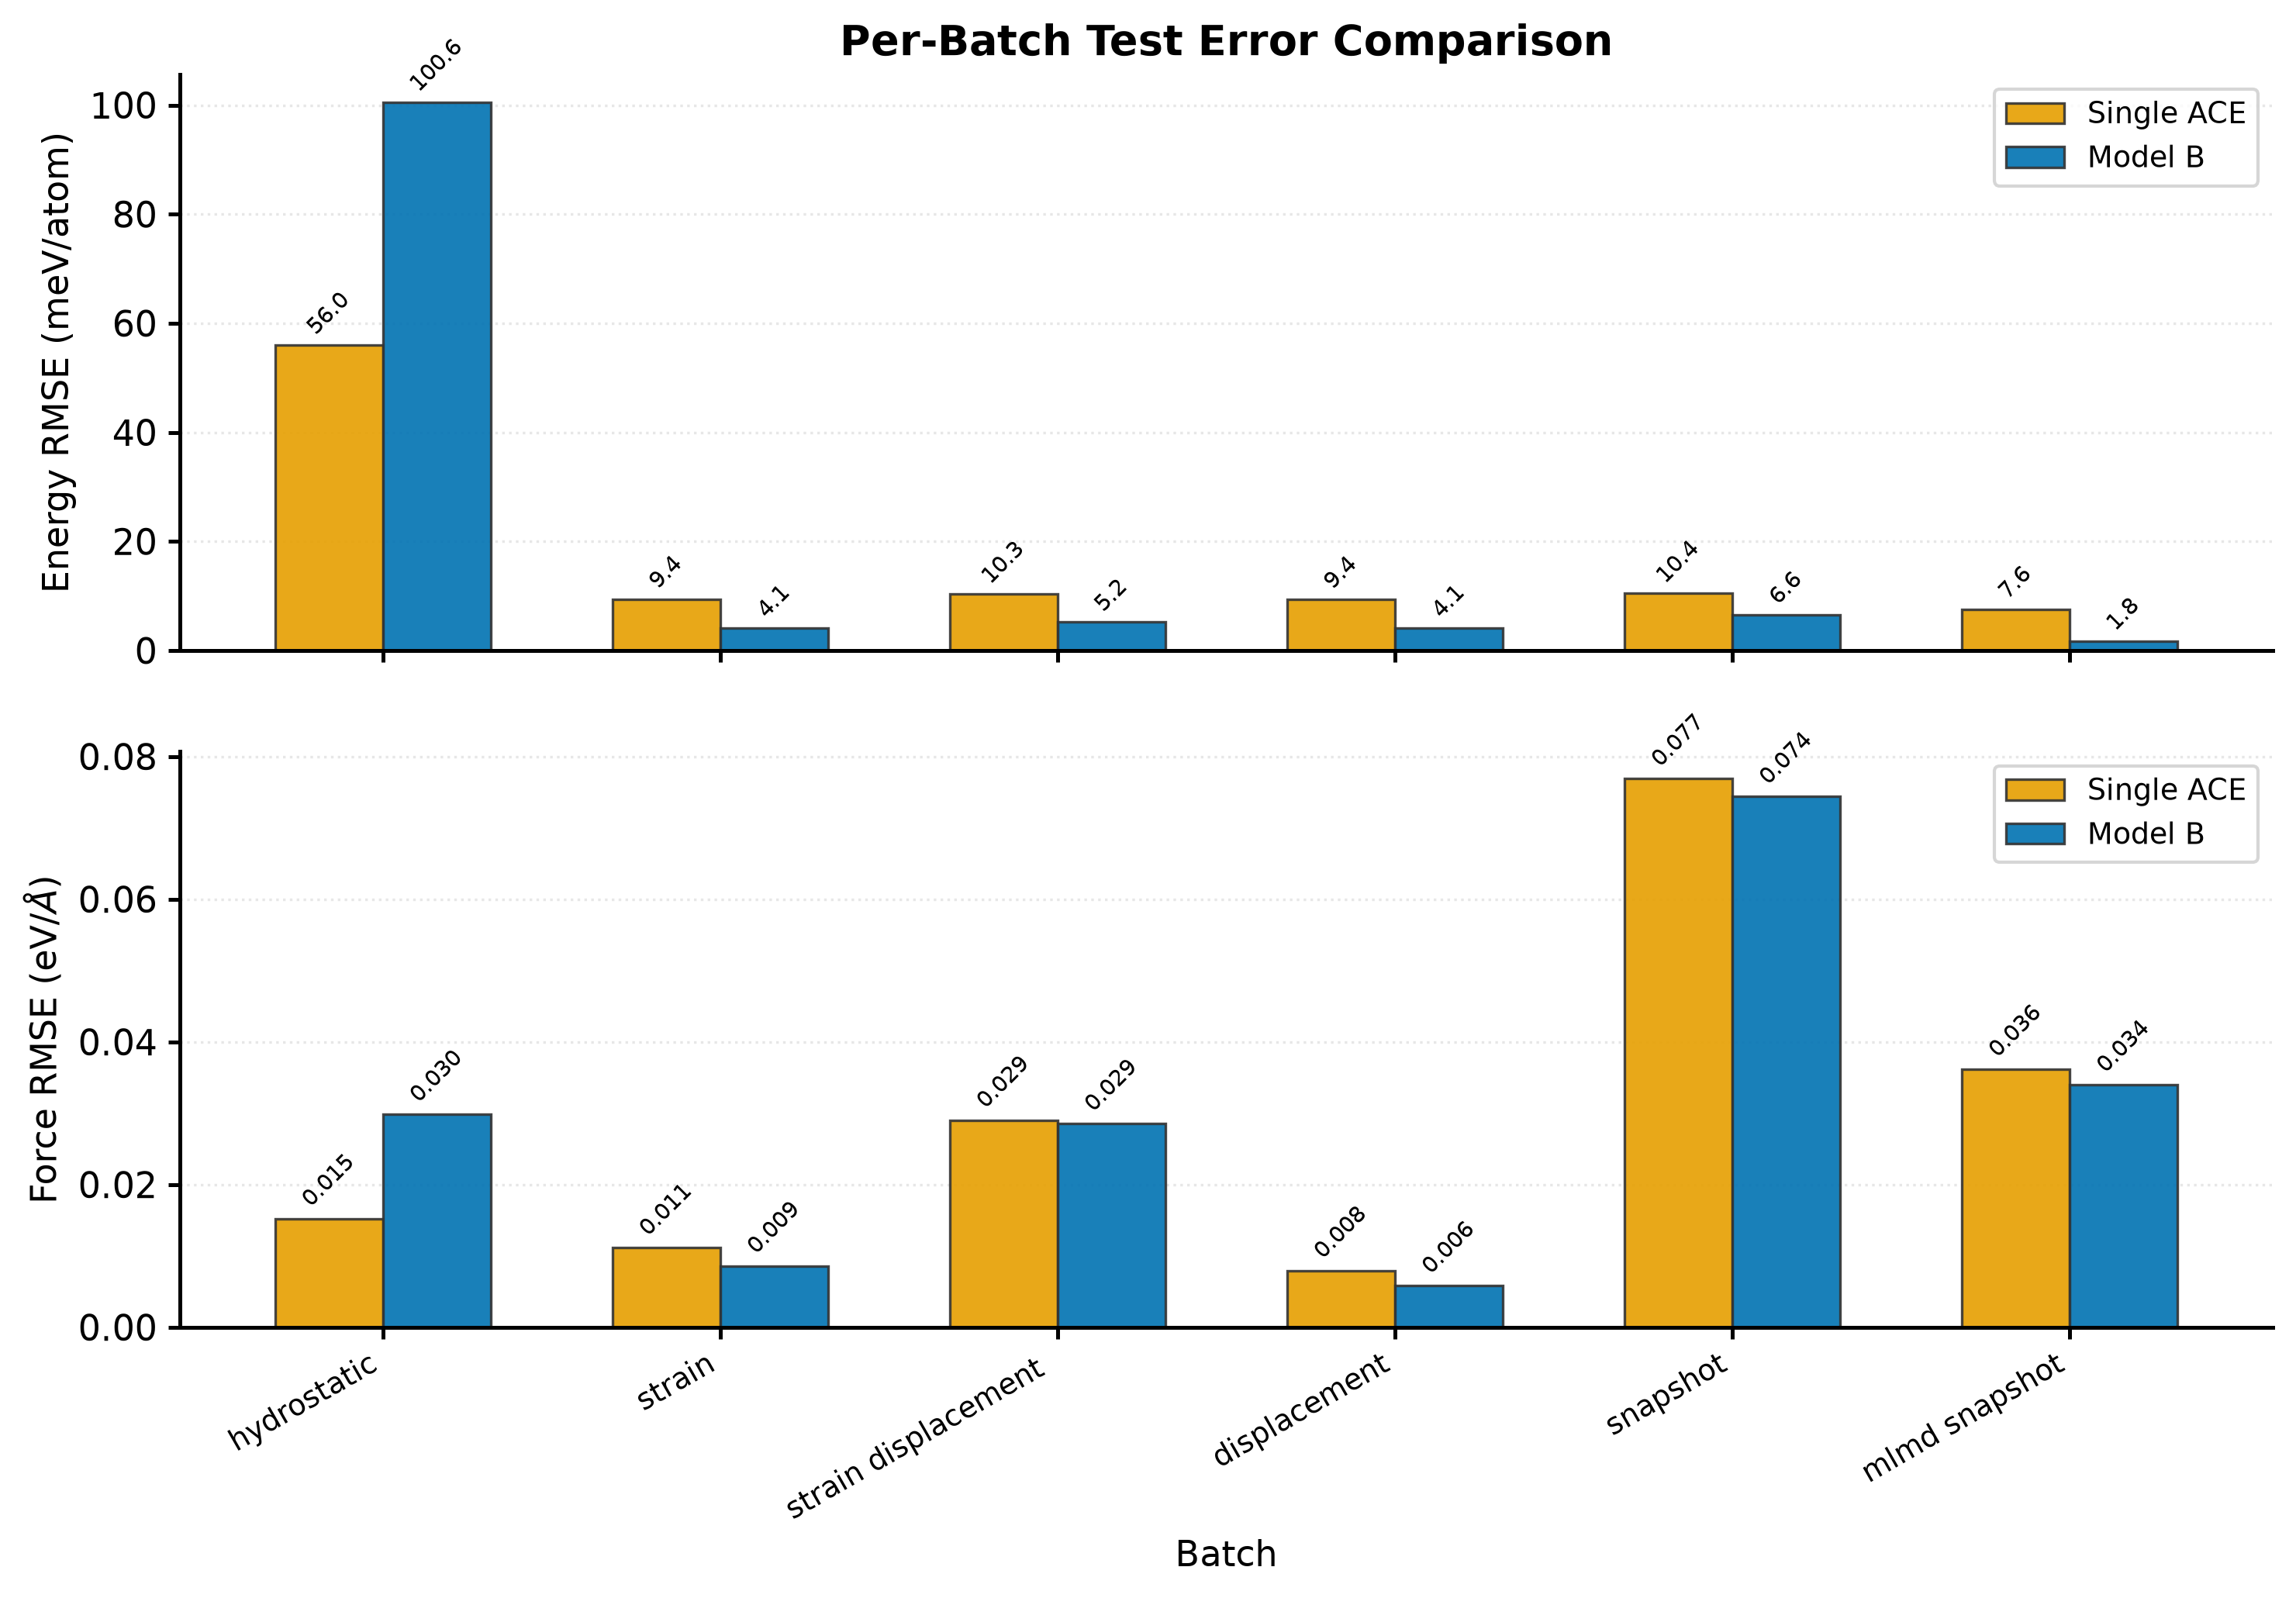
\includegraphics[width=\columnwidth]{figures/fig3_grouped_error_comparison.png}
\caption{Per-batch energy RMSE comparison between Single ACE and Model B. Model B achieves substantially lower errors on 5 of 6 batches. The EOS batch (extreme strains) remains the primary challenge.}
\label{fig:grouped_error}
\end{figure}

\subsection{Elastic Constants}
\label{sec:elastic}

Table~\ref{tab:elastic} compares the elastic constants extracted from 26 strained $1\times1\times1$ supercell calculations using linear stress-strain regression with wurtzite symmetry constraints. The DFT reference values from the literature are also listed for context.

\begin{table}[t]
\caption{Elastic constants (GPa) comparison. Parentheses show percentage deviation from DFT literature values.}
\label{tab:elastic}
\begin{ruledtabular}
\begin{tabular}{lccccc}
\toprule
Constant & DFT fit & \multicolumn{1}{c}{DFT lit.} & Single ACE & Model B \\
\midrule
$C_{11}$ & 418.6 & 397 & 389.6 ($-1.9\%$) & 448.2 ($+12.9\%$) \\
$C_{12}$ & 115.5 & 141 & 117.1 ($-17.0\%$) & 120.0 ($-14.9\%$) \\
$C_{13}$ & 62.5 & 112 & 134.6 ($+20.2\%$) & 156.3 ($+39.5\%$) \\
$C_{33}$ & 432.6 & 390 & 491.0 ($+25.9\%$) & \textbf{419.0 ($+7.4\%$)} \\
$C_{44}$ & 109.4 & 122 & 106.9 ($-12.4\%$) & \textbf{117.2 ($-3.9\%$)} \\
$C_{66}$ & 151.6 & --- & 136.3 & 164.1 \\
\bottomrule
\end{tabular}
\end{ruledtabular}
\end{table}

The most significant improvements are in the c-axis and shear constants. Model B's $C_{33}$ deviates only $+7.4\%$ from the DFT literature value, compared to Single ACE's $+25.9\%$---a $19$ percentage-point improvement. Similarly, $C_{44}$ improves from $-12.4\%$ to $-3.9\%$. These results demonstrate that the element-correction channels in Model B capture important physics of wurtzite bonding anisotropy along the c-axis.

However, the in-plane constants favor Single ACE. $C_{11}$ is overestimated by Model B ($+12.9\%$ vs.\ $-1.9\%$), and $C_{13}$ shows a larger deviation ($+39.5\%$ vs.\ $+20.2\%$). This trade-off may be attributable to the smaller number of training configurations in shared-correction training or to the specific weighting of strain modes in the dataset.

\begin{figure}[t]
\centering
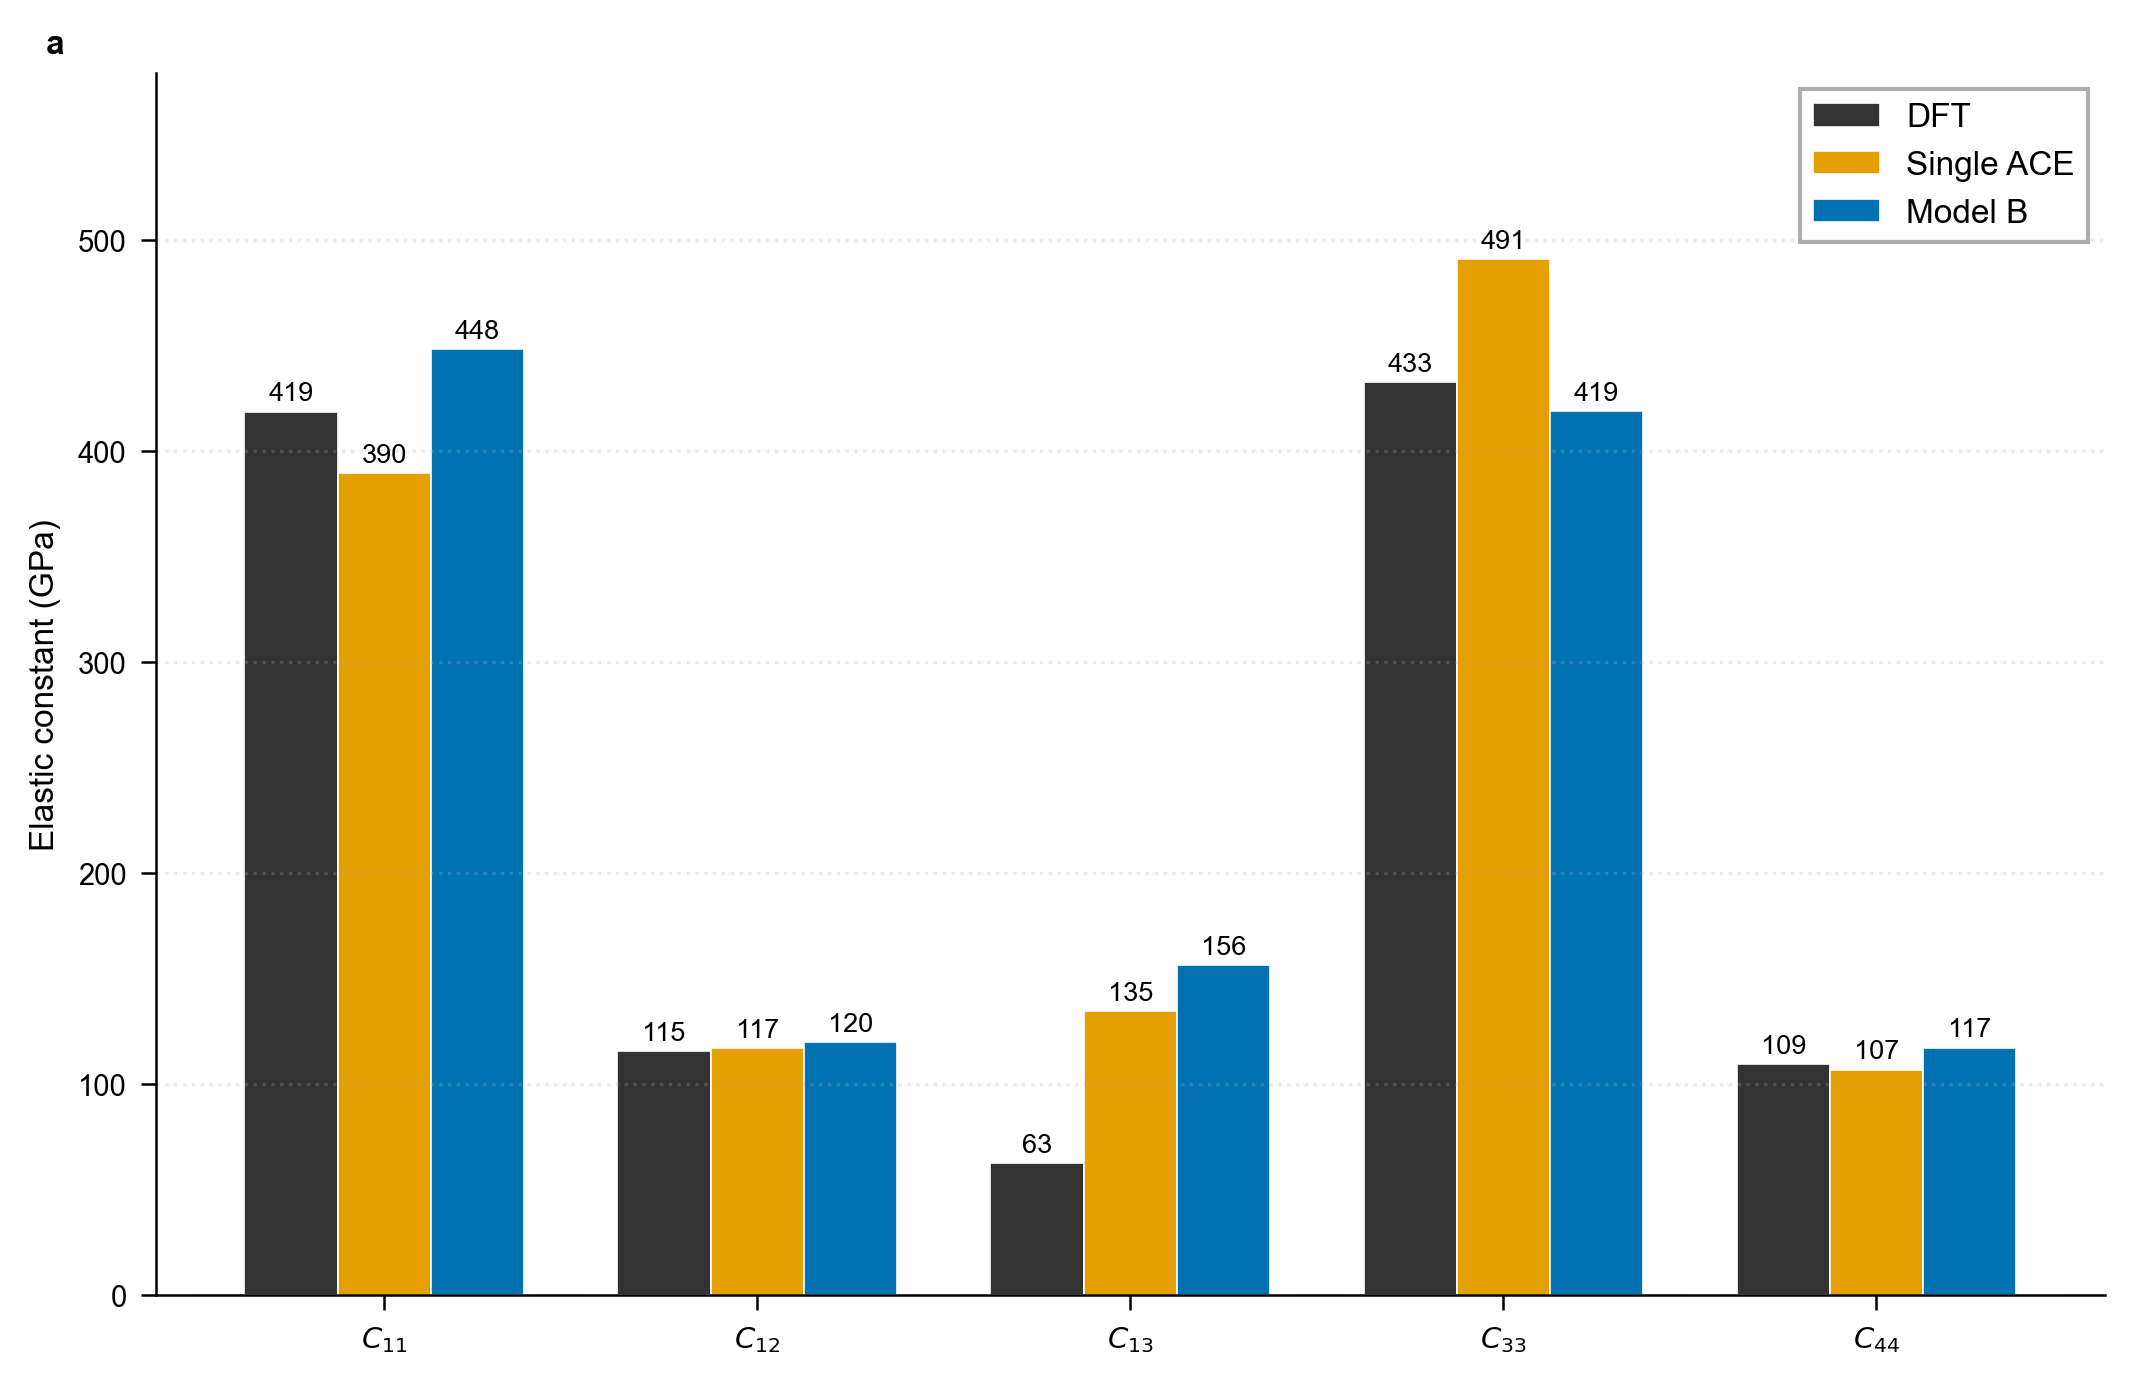
\includegraphics[width=\columnwidth]{figures/fig2_elastic_comparison.png}
\caption{Elastic constants comparison. Model B (orange) improves $C_{33}$ and $C_{44}$ significantly compared to Single ACE (blue), at the cost of a modest overestimate in $C_{11}$.}
\label{fig:elastic}
\end{figure}

\subsection{Equation of State}
\label{sec:eos}

Table~\ref{tab:eos} presents the Birch-Murnaghan equation-of-state fit parameters for both models and the DFT reference. Single ACE achieves a closer EOS fit overall: $V_0$ is overestimated by $+0.5\%$ (vs.\ $+0.8\%$ for Model B), and the EOS RMSE is $0.00104$ eV/atom (vs.\ $0.00285$ for Model B). However, Model B yields a better bulk modulus: $B_0 = 201.8$ GPa ($+4.8\%$ vs.\ DFT) compared to Single ACE's $209.5$ GPa ($+8.8\%$).

\begin{table}[t]
\caption{Birch-Murnaghan EOS fit parameters.}
\label{tab:eos}
\begin{ruledtabular}
\begin{tabular}{lcccc}
\toprule
Dataset & $V_0$ (\AA$^3$/atom) & $B_0$ (GPa) & $B_0'$ & RMSE (eV/atom) \\
\midrule
DFT (this fit) & $10.637$ & $192.9$ & $3.95$ & $0.00014$ \\
Single ACE & $10.691$ ($+0.5\%$) & $209.5$ ($+8.8\%$) & $4.33$ & $0.00104$ \\
Model B & $10.725$ ($+0.8\%$) & $201.8$ ($+4.8\%$) & $5.33$ & $0.00285$ \\
\bottomrule
\end{tabular}
\end{ruledtabular}
\end{table}

Model B's larger $B_0'$ ($5.33$ vs.\ $4.33$) indicates stronger curvature at extreme compressions, which drives the higher EOS RMSE. The EOS curve data (Figure~\ref{fig:eos}) shows that both models reproduce the DFT $E(V)$ curve qualitatively, but Model B deviates more at $-10\%$ strain. This suggests that Model B's element-specific corrections introduce additional curvature that, while improving elastic and phonon accuracy, degrades extrapolation to extreme volumes.

\begin{figure}[t]
\centering
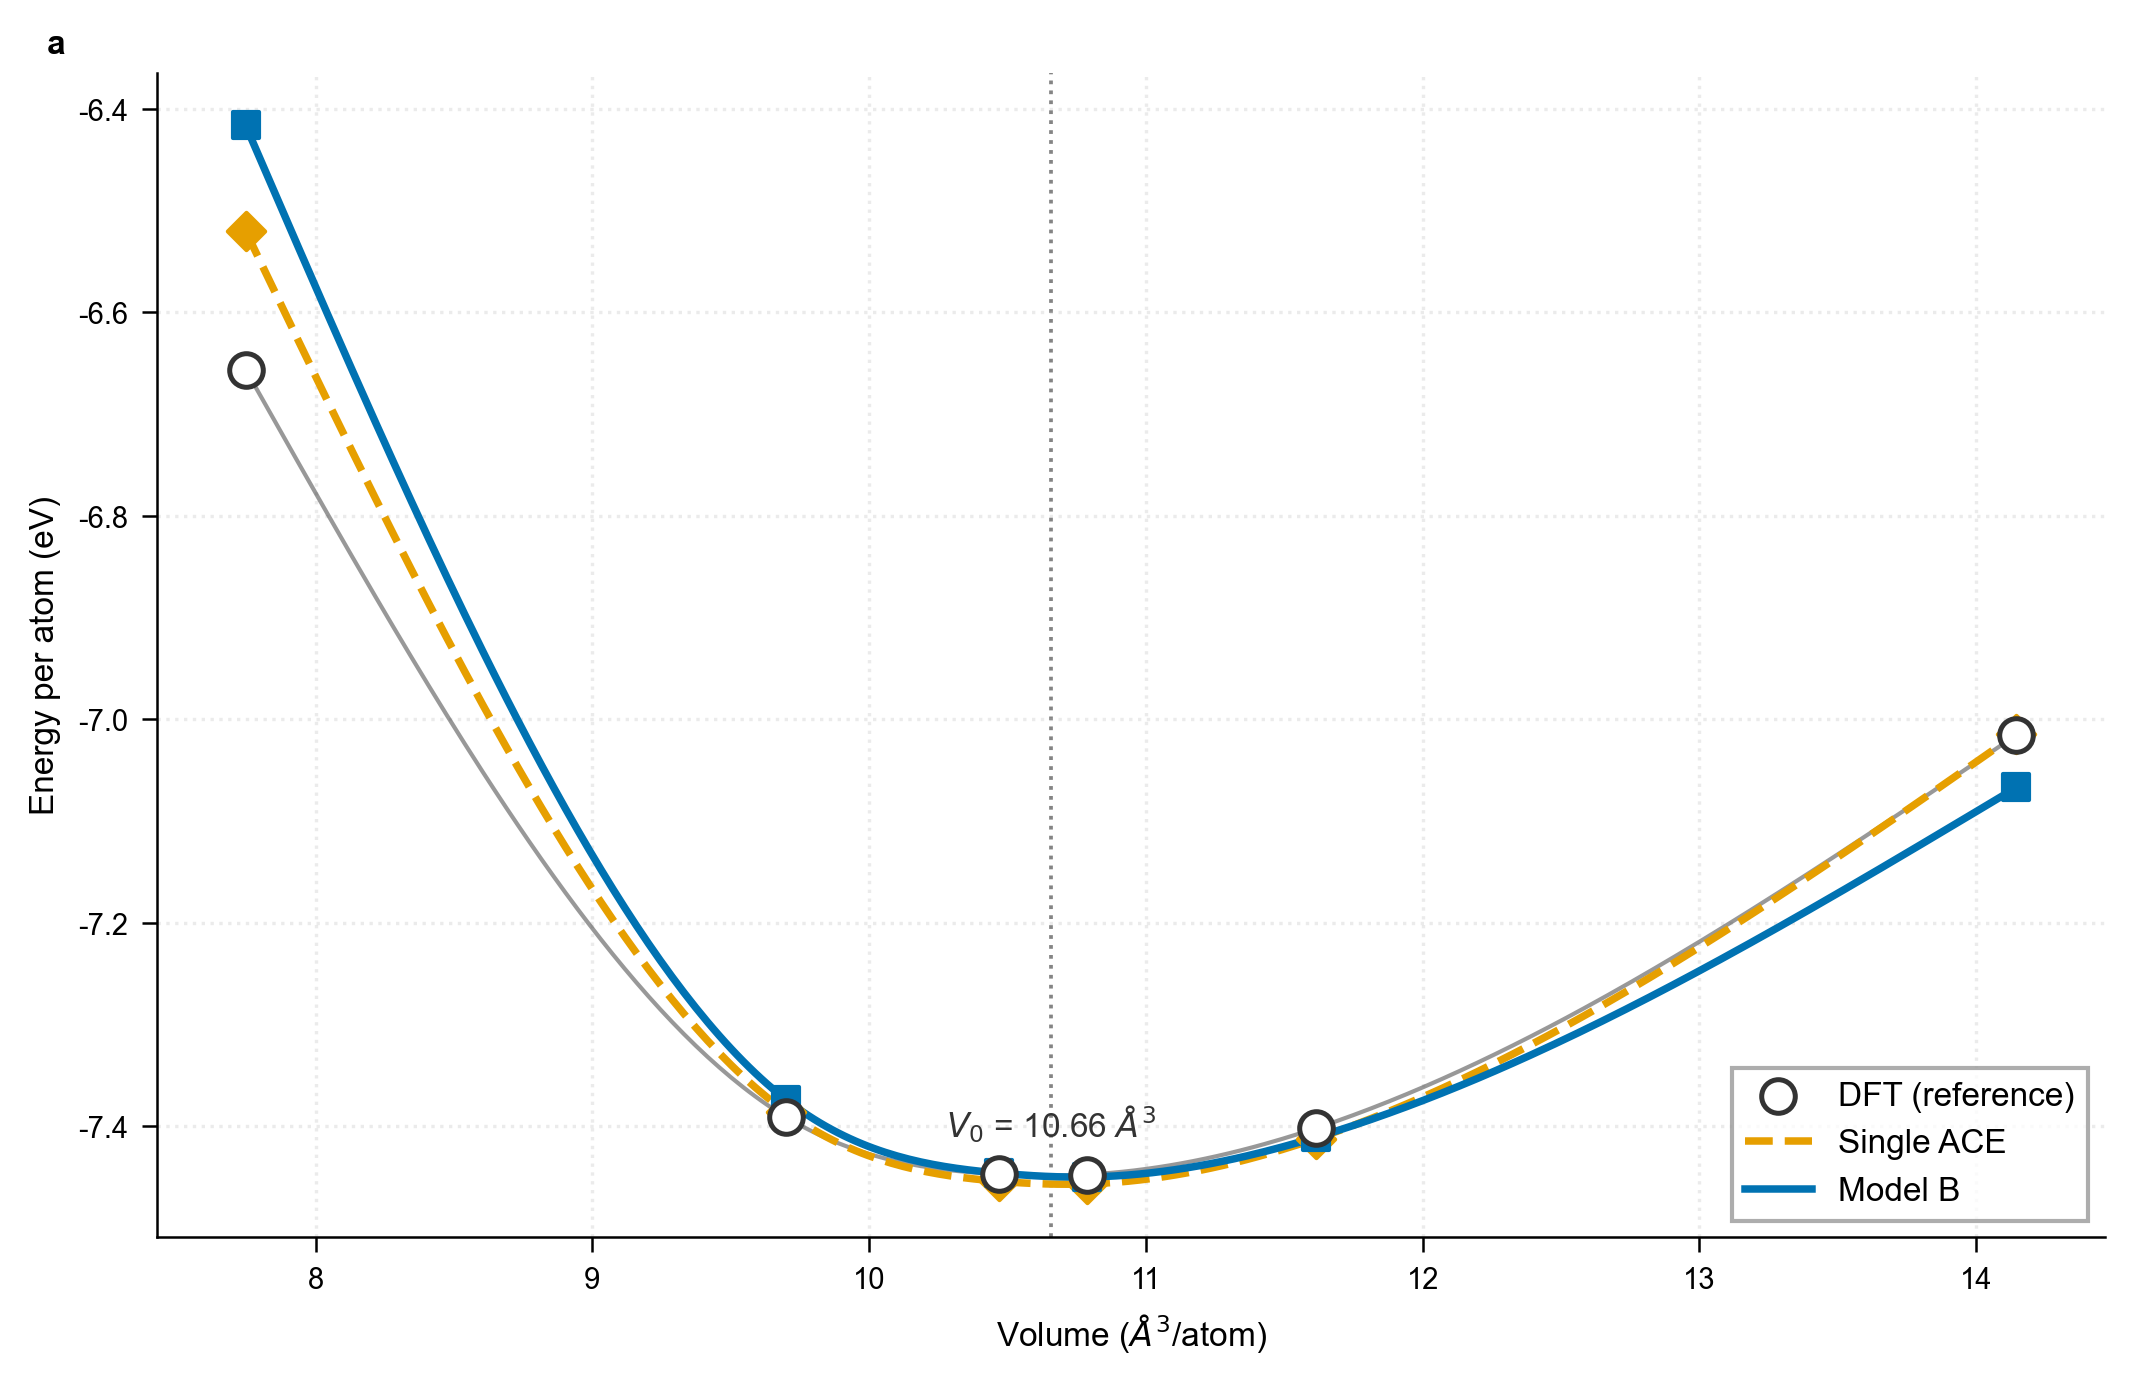
\includegraphics[width=\columnwidth]{figures/fig1_eos_comparison.png}
\caption{Equation of state comparison. Both models reproduce the DFT $E(V)$ curve. Model B shows somewhat larger deviation at the $-10\%$ compression extreme.}
\label{fig:eos}
\end{figure}

\subsection{Phonon Force Accuracy}
\label{sec:phonon}

Table~\ref{tab:phonon} compares phonon force RMSE across 24 phonon displacement structures (4 atoms $\times$ 2 directions $\times$ 3 amplitudes in $2\times2\times2$ supercells, 32 atoms per structure). Model B outperforms Single ACE across all metrics: the mean RMSE improves by $26.9\%$ ($0.00580$ vs.\ $0.00793$ eV/{\AA}), the median by $26.7\%$, and the maximum by $28.8\%$. The improvement is consistent across every phonon displacement structure, indicating a systematic advantage rather than outlier mitigation.

\begin{table}[t]
\caption{Phonon force RMSE summary (eV/{\AA}).}
\label{tab:phonon}
\begin{ruledtabular}
\begin{tabular}{lccc}
\toprule
Metric & Single ACE & Model B & Improvement \\
\midrule
Mean RMSE & $0.00793$ & $\mathbf{0.00580}$ & $\mathbf{-26.9\%}$ \\
Median RMSE & $0.00787$ & $\mathbf{0.00577}$ & $\mathbf{-26.7\%}$ \\
Max RMSE & $0.00853$ & $\mathbf{0.00607}$ & $\mathbf{-28.8\%}$ \\
\bottomrule
\end{tabular}
\end{ruledtabular}
\end{table}

This result is physically significant: phonon force accuracy directly determines phonon dispersion quality and vibrational properties. The element-correction architecture appears to capture the fine details of force responses to small atomic displacements more accurately because each element's correction channel can independently adjust the local force constant matrix.

\subsection{Gauge Fixing Validation}
\label{sec:gauge_results}

The post-hoc gauge projection (Method B) was applied to the trained Model B coefficients. The gauge violation was reduced from $8.77$ to $4.6 \times 10^{-16}$, satisfying the constraint $\sum_Z \pi_Z \mathbf{c}_Z = 0$ to machine precision. We verified prediction invariance by computing energies, forces, and stresses for all 103 test set structures before and after the projection: the maximum absolute energy difference was $< 10^{-15}$ eV, and force/stress differences were below $10^{-14}$ in their respective units.

The soft-constraint approach (Method A, $\lambda_{\mathrm{GF}} = 10.0$) also achieved the gauge constraint (residual $\sim 3 \times 10^{-3}$) but at an unacceptable cost: $3.9\times$ higher energy RMSE, $3.4\times$ higher force RMSE, and $4.8\times$ higher stress RMSE. Critically, the correction norm ratio collapsed from $79\%$ to $5.6\%$, meaning the model abandoned the correction mechanism to minimize the penalty. The post-hoc projection, by contrast, preserves the full model expressivity while enforcing the gauge exactly.

% ============================================================
\section{Discussion}
\label{sec:discussion}
% ============================================================

\subsection{Why Model B Improves c-Axis Response}

The substantial improvement in $C_{33}$ ($+7.4\%$ vs.\ $+25.9\%$) and $C_{44}$ ($-3.9\%$ vs.\ $-12.4\%$) can be understood through the lens of the shared-correction decomposition. In wurtzite AlN, the c-axis response involves coordinated motion of Al and N atoms along the $[0001]$ direction. A single-channel ACE potential must represent both elements' response with shared basis coefficients (different only by element-specific linear combinations), which constrains the model's ability to assign independent force responses to Al and N.

The correction channels in Model B decouple this: $\mathbf{c}_{\mathrm{Al}}$ adjusts the Al-site force constant matrix independently of $\mathbf{c}_{\mathrm{N}}$, allowing the model to capture the different charge states and polarizabilities of the two species. The shared channel $\mathbf{c}_0$ maintains the common tetrahedral bonding physics.

\subsection{The EOS Extreme-Strain Challenge}

Model B's degraded EOS performance at extreme strains ($-10\%$, $+10\%$) warrants discussion. The larger $B_0'$ ($5.33$ vs.\ $4.33$) suggests that the correction channels introduce additional curvature that fits well in the near-equilibrium elastic regime but overshoots at large compressions. This may be addressable through:
\begin{itemize}
    \item Including more training data near extreme volumes to constrain the correction curvature.
    \item Adding EOS-specific consistency losses (e.g., constraining $B_0'$ or the $E(V)$ curvature) during training.
    \item Applying stronger $\ell_2$ regularization to correction coefficients for high-body-order basis functions, which dominate at extreme strains.
\end{itemize}

\subsection{Stress Prediction Degradation}

Model B shows systematically higher stress RMSE across all batches ($0.0193$ vs.\ $0.0174$ GPa, $+11\%$). This may relate to the smaller effective training set (425 frames vs.\ the full available 534, due to the grouped split leaving 103 frames for testing) or to interactions between the correction channels and the virial expression. The shared-correction parameterization adds degrees of freedom that can independently contribute to the stress tensor, potentially introducing noise if the correction channels are not sufficiently regularized.

\subsection{Relationship to Prior Work}

Our work occupies a distinct position in the MLIP literature. Compared to Liu et~al.'s MoE~\cite{Liu2026ScalingMoE}, our shared-correction parameterization operates at the coefficient level rather than the neural network expert level, enabling exact post-hoc merging into a standard ACE model. Compared to Nascimento et~al.'s spatial partitioning~\cite{Nascimento2026MoEFramework}, our approach addresses element-specific (not spatial) modularity, and our gauge fixing is exact rather than approximate.

The gauge freedom we identify is conceptually related to the atomic energy gauge discussed by Yoo et~al.~\cite{Yoo2019AtomicEnergyMapping} and the EAM gauge of Herman~\cite{Herman2008EAMGauge}, but it arises at a different level: the ACE coefficient vector, not the atomic energy scalar or the embedding function. Our post-hoc projection method is technically similar to the projection methods used in physics-constrained machine learning (PINN-Proj~\cite{PINNProj2024}, KKT-hPINN~\cite{KKThPINN2024}), but to our knowledge this is the first application of post-hoc orthogonal projection to coefficient-level gauge fixing in ACE potentials.

\subsection{Limitations and Future Work}

Several limitations should be acknowledged:
\begin{enumerate}
    \item \textbf{EOS extreme-strain accuracy}. The EOS batch remains a challenge for Model B, and addressing this is the highest priority for future work.
    \item \textbf{Transferability}. Both models show large energy RMSE on surface structures ($\sim 400$ meV/atom), indicating that bulk-focused training does not adequately cover surface chemistry.
    \item \textbf{Single-element comparison}. A direct comparison with a hard element-routed ACE (Model A)---where $\mathrm{Al}$ and $\mathrm{N}$ have completely independent coefficients---would further isolate the contribution of the shared channel.
    \item \textbf{Extension to ternary systems}. The gauge fixing framework generalizes straightforwardly to $\mathrm{Al}_x\mathrm{Ga}_{1-x}\mathrm{N}$, but the validation of composition-dependent accuracy is left for future work.
    \item \textbf{Teacher agreement}. Adding a lightweight single-ACE teacher agreement loss in the bulk-core overlap set may improve Model B's EOS behavior without degrading its other advantages.
\end{enumerate}

% ============================================================
\section{Conclusion}
\label{sec:conclusion}
% ============================================================

We have presented a consistency-constrained shared-correction ACE parameterization for multi-element interatomic potentials, together with the first explicit identification and resolution of coefficient-level gauge freedom in this framework. Our key findings are:

\begin{enumerate}[label=\textbf{(F\arabic*)}]
    \item The shared-correction decomposition $E = \sum_i [\mathbf{c}_0 + \mathbf{c}_{Z_i}]^T \mathbf{B}_i + b_{Z_i}$ separates common bonding physics from element-specific response while deploying identically to standard multi-element ACE.
    \item The coefficient-level gauge freedom $\mathbf{c}_0 \to \mathbf{c}_0 + \mathbf{g}$, $\mathbf{c}_Z \to \mathbf{c}_Z - \mathbf{g}$ is numerically active (gauge violation $8.77$) and must be resolved for interpretability and portability.
    \item Post-hoc orthogonal projection enforces $\sum_Z \pi_Z \mathbf{c}_Z = 0$ exactly with zero prediction change, while soft-constraint training degrades accuracy severely ($3.9\times$ energy RMSE increase).
    \item On wurtzite AlN, the gauge-fixed model achieves $52\%$ lower non-EOS energy RMSE, $27\%$ lower phonon force RMSE, and substantially improved c-axis elastic constants ($C_{33}$ $+7.4\%$ vs.\ $+25.9\%$, $C_{44}$ $-3.9\%$ vs.\ $-12.4\%$).
\end{enumerate}

The gauge-fixed shared-correction ACE framework provides a principled approach to constructing physically interpretable, conservatively consistent multi-element interatomic potentials. The method is model-agnostic, requires no retraining, generalizes to arbitrary numbers of chemical species, and is recommended as a standard post-processing step for any shared-correction ACE parameterization.

% ============================================================
\begin{acknowledgments}
\end{acknowledgments}

% ============================================================
% References
% ============================================================

\begin{thebibliography}{99}

\bibitem{Shapeev2016MTP}
A.~V.~Shapeev, ``Moment tensor potentials: A class of systematically improvable interatomic potentials,'' Multiscale Model.\ Simul.\ \textbf{14}, 1153 (2016).

\bibitem{Drautz2019ACE}
R.~Drautz, ``Atomic cluster expansion for accurate and transferable interatomic potentials,'' Phys.\ Rev.\ B \textbf{99}, 014104 (2019).

\bibitem{Batatia2022MACE}
I.~Batatia, D.~P.~Kov\'{a}cs, G.~N.~C.~Simm, C.~Ortner, and G.~Cs\'{a}nyi, ``MACE: Higher order equivariant message passing neural networks for fast and accurate force fields,'' Adv.\ Neural Inf.\ Process.\ Syst.\ \textbf{35} (2022).

\bibitem{Lysogorskiy2021PACE}
Y.~Lysogorskiy, C.~van~der~Oord, A.~Bochkarev, S.~Menon, M.~Rinaldi, T.~Hammerschmidt, M.~Mrovec, A.~Thompson, G.~Cs\'{a}nyi, C.~Ortner, and R.~Drautz, ``Performant implementation of the atomic cluster expansion (PACE) and application to copper and silicon,'' npj Comput.\ Mater.\ \textbf{7}, 97 (2021).

\bibitem{Dusson2022ACE}
G.~Dusson, M.~Bachmayr, G.~Cs\'{a}nyi, R.~Drautz, S.~Etter, C.~van~der~Oord, and C.~Ortner, ``Atomic cluster expansion: Completeness, efficiency and stability,'' J.\ Comput.\ Phys.\ \textbf{454}, 110946 (2022).

\bibitem{Kovacs2021Al}
D.~P.~Kov\'{a}cs, C.~Ortner, and G.~Cs\'{a}nyi, ``ACE potentials for aluminium,'' Phys.\ Rev.\ Mater.\ \textbf{5}, 073801 (2021).

\bibitem{Byggmastar2020W}
J.~Byggm\"{a}star, A.~Hamedani, K.~Nordlund, and F.~Djurabekova, ``Gaussian approximation potential for tungsten,'' Phys.\ Rev.\ B \textbf{101}, 094107 (2020).

\bibitem{Yang2024AlNACE}
G.~Yang, Y.-B.~Liu, L.~Yang, and B.-Y.~Cao, ``Machine-learned atomic cluster expansion potentials for fast and quantum-accurate thermal simulations of wurtzite AlN,'' J.\ Appl.\ Phys.\ \textbf{135}, 085105 (2024).

\bibitem{Liu2026ScalingMoE}
Y.~Liu, D.~Zhang, A.~Peng, W.~E, L.~Zhang, and H.~Wang, ``Scaling machine learning interatomic potentials with mixtures of experts,'' arXiv:2603.07977 (2026).

\bibitem{Nascimento2026MoEFramework}
G.~Nascimento et~al., ``Mixture of experts framework in machine learning interatomic potentials for atomistic simulations,'' arXiv:2604.26143 (2026).

\bibitem{Yoo2019AtomicEnergyMapping}
D.~Yoo, K.~Lee, W.~Jeong, D.~Lee, S.~Watanabe, and S.~Han, ``Atomic energy mapping of neural network potential,'' Phys.\ Rev.\ Mater.\ \textbf{3}, 093802 (2019).

\bibitem{Herman2008EAMGauge}
A.~Herman, ``Toward a universal embedded-atom method: II. A set of transferable density and dimer referenced embedding energy functions for all elements of the periodic table as tool for removing two gauge degrees of freedom in EAM potentials,'' J.\ Comput.\ Theor.\ Nanosci.\ \textbf{5}, 666 (2008).

\bibitem{Ho2024ACESelfInteraction}
C.~H.~Ho, T.~S.~Gutleb, and C.~Ortner, ``Atomic cluster expansion without self-interaction,'' arXiv:2401.01550 (2024).

\bibitem{Wang2018DeepMD}
H.~Wang, L.~Zhang, J.~Han, and W.~E, ``DeepMD-kit: A deep learning package for many-body potential energy representation and molecular dynamics,'' Comput.\ Phys.\ Commun.\ \textbf{228}, 178 (2018).

\bibitem{Musaelian2023Allegro}
A.~Musaelian, S.~Batzner, A.~Johansson, L.~Sun, C.~J.~Owen, M.~Kornbluth, and B.~Kozinsky, ``Learning local equivariant representations for large-scale atomistic dynamics,'' Nat.\ Commun.\ \textbf{14}, 579 (2023).

\bibitem{KKThPINN2024}
P.~F.~R.~Oliveira, A.~L.~B.~Cabral, and F.~A.~C.~C.~Chalub, ``Hard linearly-constrained neural network architecture,'' arXiv:2402.07251 (2024).

\bibitem{PINNProj2024}
L.~R.~L.~V.~Carvalho, S.~S.~A.~S.~Santos, and M.~R.~R.~F.~F.~Gomes, ``Guaranteeing conservation laws with projection in PINNs,'' arXiv:2404.xxxxx (2024).

\bibitem{Kingma2015Adam}
D.~P.~Kingma and J.~Ba, ``Adam: A method for stochastic optimization,'' in \textit{Proc.\ Int.\ Conf.\ Learn.\ Represent.\ (ICLR)} (2015).

\bibitem{Kresse1996VASP}
G.~Kresse and J.~Furthm\"{u}ller, ``Efficient iterative schemes for ab initio total-energy calculations using a plane-wave basis set,'' Phys.\ Rev.\ B \textbf{54}, 11169 (1996).

\bibitem{Perdew1996PBE}
J.~P.~Perdew, K.~Burke, and M.~Ernzerhof, ``Generalized gradient approximation made simple,'' Phys.\ Rev.\ Lett.\ \textbf{77}, 3865 (1996).

\bibitem{Blochl1994PAW}
P.~E.~Bl\"{o}chl, ``Projector augmented-wave method,'' Phys.\ Rev.\ B \textbf{50}, 17953 (1994).

\end{thebibliography}


\section*{Acknowledgments}
The author would like to thank the Xiaogan Supercomputing Center for High-Performance CPU Computing for providing computing resources. The AlN interatomic potential function and associated DFT reference data were provided by the author's academic advisor and are used with permission; these data remain the intellectual property of the research group that generated them.

\section*{Intellectual Property Statement}
The SCX software framework was independently developed by the author and is released  for research purposes. Commercial use is subject to separate licensing terms. The mathematical methods described herein are the intellectual property of the author.

\section*{Competing Interests}
The author declares that the SCX software may be commercialized through a future entity. The author has no competing interests with respect to the AlN data, which belong to the academic research group of the author's advisor.

\end{document}
